\entry{Semana del 13/10/2025.} 

\section{Ordinal analysis} 

Parte de la semana pasada y esta la estuve dedicando a intentar analizar nuestras series temporales para turbulencia de ondas con un método para sistemas no lineales llamado \textit{ordinal analysis}, utilizando un paquete de Python llamado \textit{ordpy}. De momento no voy a entrar demasiado en detalle ya que los resultados fueron no demasiado concluyentes. 

Básicamente todo se reduce a elegir los llamados parámetros de embedding, que son la longitud $\tau$ y la dimensión $d$. Sin embargo, no hay criterios bien establecidos en la literatura para su elección. El procedimiento después consiste en tomar de la serie temporal los $d$ puntos consecutivos separados $\tau$ y ver qué patrón forman. Por ejemplo, si la serie fuese (1.1, 7.2, 5.4) su patrón asociado sería (132). 

Luego con la serie de patrones se puede calcular la probabilidad de cada uno, y con éstas su entropía y complejidad estadística. La cuestión es que varían muchos los puntos en el plano HC según la elección de estos parámetros (acá tenemos mucha libertad para elegirlos ya que nuestras series temporales son muy largas). 


Por ejemplo más abajo vemos lo que pasa al variar $\tau$ para una de las señales dejando $d$ fijo. La idea original era asociar ese comportamiento a distintas escalas del flujo pero siempre hace cosas parecidas (haya o no por ejemplo intermitencia). 

\begin{figure}[th!]
	\centering
	\includegraphics[width=0.51467\linewidth]{"Figures/13_10_2025/Variar_tau_0_6_Hz_k_noise"} %  }  } 
\caption{Variar el parámetro $\tau$ para la señal de la banda entre 0 y 6 Hz con $d$=6.}
\label{fig:variartau06hzknoise-}
\end{figure}

Y después para el caso en que dejamos $\tau$ = 5 fijo y variamos la dimensión $d$, también se mueve bastante, cambiando incluso de regiones en el planos HC. 

\begin{figure}[th!]
	\centering
	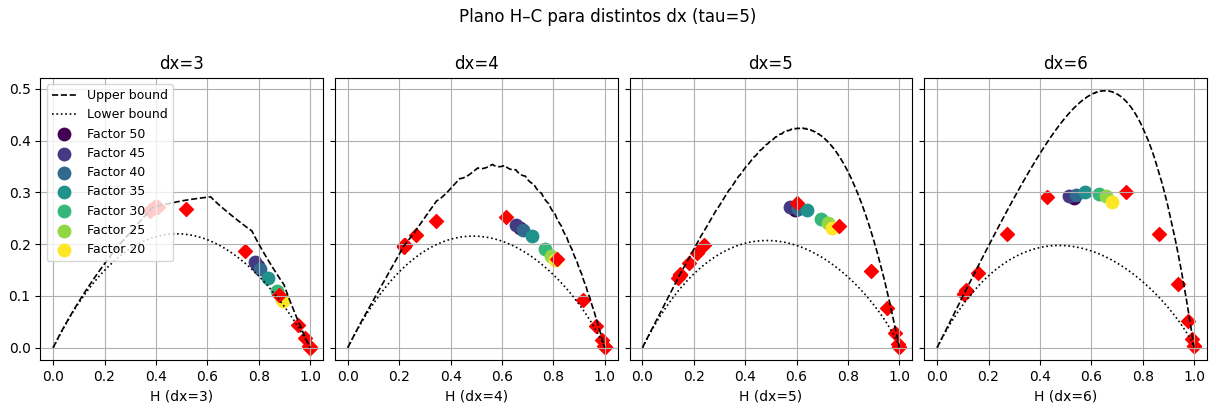
\includegraphics[width=0.718\linewidth]{Figures/13_10_2025/Variar_dx}
	\caption{Varir la dimensión $d$ dejando $\tau=5$ fijo para todas las series temporales de la banda entre 0 y 4 Hz.}
	\label{fig:variardx}
\end{figure}

